\documentclass[landscape,a0paper,fontscale=0.285]{baposter}

\usepackage{graphicx}
\usepackage{listings}
\graphicspath{{figures/}}

\usepackage{amsmath}
\usepackage{amssymb}

\usepackage{booktabs}
\usepackage{enumitem}
\usepackage{palatino}
\usepackage[font=small,labelfont=bf]{caption}

\usepackage{multicol}
\setlength{\columnsep}{1.5em}
\setlength{\columnseprule}{0mm}

\usepackage{tikz}
\usetikzlibrary{shapes,arrows}

\newcommand{\compresslist}{
\setlength{\itemsep}{1pt}
\setlength{\parskip}{0pt}
\setlength{\parsep}{0pt}
}

\setlength\fboxsep{4.0pt}
\setlength\fboxrule{1.0pt}

\begin{document}
\pretolerance=10000
\tolerance=2000 
\emergencystretch=10pt

\begin{poster}
{
  %% View grid for debugging.
  grid=false,
  %% Column specification.
  columns=4,
  colspacing=1em,
  %% Poster coloring, taken from WPI's poster template.
  bgColorOne=white!80!blue,
  bgColorTwo=white!80!green,
  %% Border 
  borderColor=black,
  headerColorOne=white,
  headerColorTwo=white,
  headerFontColor=blue,
  boxColorOne=white,
  textborder=roundedsmall,
  eyecatcher=true,
  headerborder=open,
  headerheight=0.22\textheight,
  headershape=smallrounded,
  headershade=plain,
  headerfont=\Large\bf\textsc, %Sans Serif
  textfont={\setlength{\parindent}{1.5em}},
  boxshade=plain,
  borderColor=black,
  background=shadetb,
  linewidth=2pt
}
% University logo
{
  
\includegraphics[width=0.2\linewidth]{wpi_logo.png}
} 
% Title
{\huge Software Similarity Detection With \textit{Checksims}\\[0.15em]
  \large Improvements to Algorithmic Comparisons and Usability}
% Authors
  {\large Theodore Meyer and Michael Andrews}
% Eye catcher
{
  
\includegraphics[width=0.2\linewidth]{checksims_logo.png}
}

\headerbox{Motivation and Objectives}{name=M-and-O, column=0, row=0, span=1}{
    \noindent \textbf{Motivations:}
    \begin{itemize}
        \item The Smith-Waterman algorithm is flawed in that it is not able to detect renaming variables and reordering code.
        \item \textit{CheckSims} is difficult to use in its commandline only form for many course staff. 
    \end{itemize}

    \noindent \textbf{Objectives:}
    \begin{itemize}
        \item Design and implement an AST Similarity detection algorithm that is \textit{at least} as powerful as Smith-Waterman, and hopefully better.
        \item Design an archive system for \textit{CheckSims} so that assignments can be bundled together in a single file
        \item Build an interoperability layer with \textit{Turnin} so that detection can be done more quickly.
        \item Create a User Interface for \textit{CheckSims} so that course staff who are unable to use a command line have a way to use \textit{CheckSims}
    \end{itemize}
}

\headerbox{AST Approach}{name=Approach, column=0, row=.65, span=1}{
    \noindent \textbf{An AST (Abstract Syntax Tree) is a simple data structure for representing source code}
    \noindent \begin{itemize}
        \item The \textit{ANTLR} parser generator was used to create parsers for C, C++, Java, and Python, all of which were translated into our universal AST representation.
        \item ASTs are transformed into hashmaps so that intersecting keysets can be found; each hashmap is cached for better runtime.
    \end{itemize}
}

\headerbox{AST Comparison Algorithm}{name=ast-comparison, column=1, span=1}{
    \lstinputlisting{./pseudo.code}
}

\headerbox{AST Comparison vs Smith-Waterman}{name=algocompare, column=1, row=.64, span=2} {
  \parbox[c][0.28\linewidth][t]{0.60\linewidth}{
    \fbox{
      
\includegraphics[width=0.9\linewidth]{ast.png}
    }
  }
  \parbox[c][0.2\linewidth][t]{0.30\linewidth}{
    AST versus Smith-Waterman comparison on variable renaming. AST based methods
    identify a perfect match, while Smith-Waterman returns a weak similarity.
  }
}

\headerbox{Future Work}{name=futurework, column=3, row=.64, span=1} {

  Future work for \textit{Checksims} might include:
  \begin{itemize}
  \item Support for more languages using the AST comparison algorithms.
  \item Printable reports detailing the line-by-line similarities of documents.
  \item Further integration with existing assignment submission systems.
  \item Improvements to the GUI user experience.
  \end{itemize}
}

\headerbox{GUI Approach}{name=approach2, column=2, span=2} {
    Because \textit{CheckSims} is written in java, we chose to use Java Swing for
    developing the GUI. The GUI captures all of the core options provided by the
    core \textit{Checksims} system.
    The \textit{Checksims} GUI has the following significant features:
    \begin{itemize}
    \item A startup menu for selecting the files and comparision method to use.
    \item A loading screen that displays useful information about the progress of
      each run.
    \item A results screen that allows users to search, sort, browse, and inspect
      the similarity matrix.
    \end{itemize}
  
    Given the steep learning curve for using the command line interface, this GUI
    makes \textit{Checksims} significantly more usable.

    \parbox[c][0.35\linewidth][b]{0.48\linewidth}{
      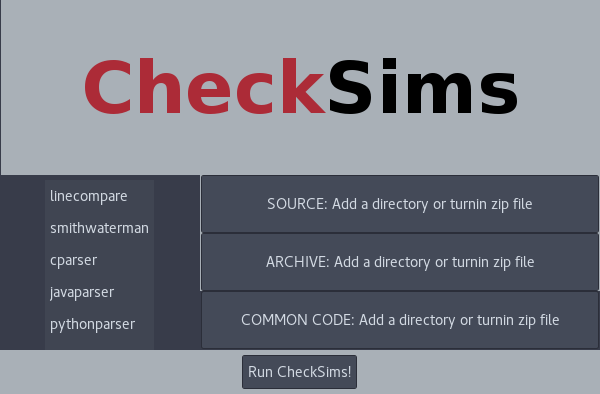
\includegraphics[width=0.9\linewidth]{initial_run.png} \\
      The lobby menu with all available options.
    }
    \parbox[c][0.35\linewidth][b]{0.48\linewidth}{
      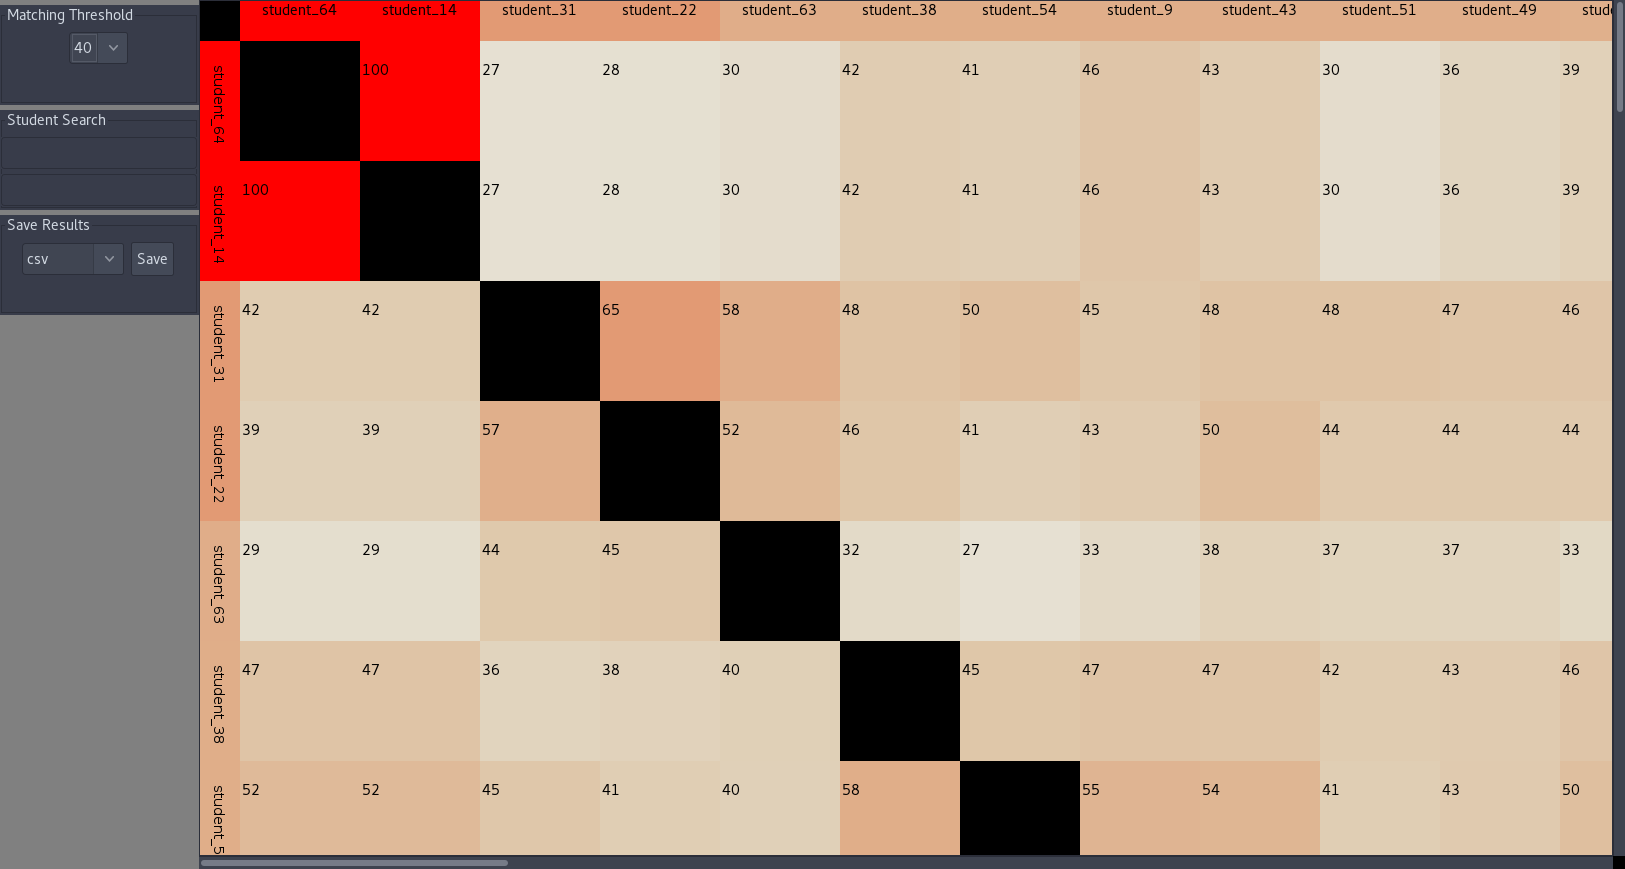
\includegraphics[width=0.9\linewidth]{demo_screen.png} \\
      The similarity comparison matrix view \\
      and results screen.
    }
}


\end{poster}

\end{document}
